%%%%%%%%%%%%%%%%%%%%%%%%%%%%%%%%%%%%%%%%%%%%%%%%%%%%%%%%%%%%%%%%%
\begin{frame}[fragile]
\frametitle{\textbf{\textcolor{orange}{Descartes' rule of sign}}}

\begin{drs}[DRS]
Consider a univariate polynomial $P\in\mathbb{R}[X]$ and the sequence 
$(a_n)$ of its non-zero coefficients. Let $c$ be the number of sign changes 
of the sequence $(a_n)$. Then the number of positive roots of $P$ is at most $c$.
\end{drs}

\begin{gp}
If we consider the previous rule of signs and 
count the roots with their multiplicities, 
then the number of positive real roots of $P$ 
has the same parity as $c$.
\end{gp}

This rule can also be used to determine the number of negative real roots of polynomials.

\end{frame}
%%%%%%%%%%%%%%%%%%%%%%%%%%%%%%%%%%%%%%%%%%%%%%%%%%%%%%%%%%%%%%%%%

%%%%%%%%%%%%%%%%%%%%%%%%%%%%%%%%%%%%%%%%%%%%%%%%%%%%%%%%%%%%%%%%%
\begin{frame}[fragile]
\frametitle{\textbf{\textcolor{orange}{Intermediate values theorem}}}

\begin{ivt}[IVT]
If $f$ is a real-valued continuous function on the interval $[a, b]$ and $M$ is a number between $f(a)$ and $f(b)$, then there exists $c\in [a, b]$ such that we have $f(c) = M$.
\end{ivt}

\begin{center}
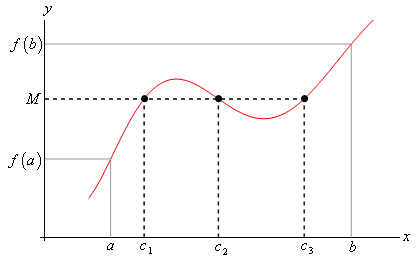
\includegraphics[scale=0.25]{TIV.png}
\end{center}

In particular if $M = 0$, then there exists $c\in [a, b]$ such that $f(c) = 0$ holds.

\end{frame}
%%%%%%%%%%%%%%%%%%%%%%%%%%%%%%%%%%%%%%%%%%%%%%%%%%%%%%%%%%%%%%%%%

%%%%%%%%%%%%%%%%%%%%%%%%%%%%%%%%%%%%%%%%%%%%%%%%%%%%%%%%%%%%%%%%%
\begin{frame}[fragile]
\frametitle{\textbf{\textcolor{orange}{Horner's method}}}

\begin{itemize}
\item We want to evaluate the following polynomial :
$$P(X) = \sum_{i=0}^{n} a_i\, X^i = a_0 + a_1\, X + a_2\, X^2 + \cdots + a_n\, X^n$$

\begin{block}{}
A better way to evaluate it is to use \textcolor{red}{\textbf{Horner's method}}, that is, represents $P$ in the following form :
$$\textcolor{darkgreen}{P(X) = a_0 + X\, \left(a_1 + X\, \left(a_2 + X\,\left(\cdots \left(a_{n-1} + \left(a_n\, X\right)\cdots \right)\right)\right)\right)}$$
\end{block}

\item \textcolor{blue}{\underline{\textbf{\textit{costs of operations :}}}} $\Theta(n)$ for \textit{Horner's method}, $\Theta(n^2)$ for naive method.
\end{itemize}

\end{frame}
%%%%%%%%%%%%%%%%%%%%%%%%%%%%%%%%%%%%%%%%%%%%%%%%%%%%%%%%%%%%%%%%%

%%%%%%%%%%%%%%%%%%%%%%%%%%%%%%%%%%%%%%%%%%%%%%%%%%%%%%%%%%%%%%%%%
\begin{frame}[fragile]
\frametitle{\textbf{\textcolor{orange}{Example of real root search}}}

Let's consider \textcolor{darkgreen}{$P(X) = X^3 + 3\, X^2 - X - 2$} : $c = 1$ so $P$ has $1$ positive root. \\
$P(-X) = -X^3 + 3\, X^2 + X - 2$ : $c = 2$ so $P$ has $2$ or $0$ negative roots.\\
\vspace{4mm}
$P(-1) = 1$, $\lim_{X \to -\infty} P(X) = -\infty$ $\Rightarrow$ $\exists r_{1}\in ]-\infty; -1[\;$ | $P(r_1) = 0$ \\
$\Rightarrow$ $P$ has $2$ negative roots.\\
\vspace{4mm}
\textcolor{blue}{\underline{Let's use the \textit{IVT} for $M = 0$ :}} \\
The following evaluations of $P$ can be done using the \textit{Horner's method}.\\
As $P(-1) =  1$ and $P(-2) = -2$, then \textcolor{red}{$r_1\in ]-2, -1[$}.\\
As $P(0)  = -2$ and $P(-1) =  1$, then \textcolor{red}{$r_2\in ]-1,  0[$}.\\
As $P(0)  = -2$ and $P(1)  =  1$, then \textcolor{red}{$r_3\in ] 0,  1[$}.

\end{frame}
%%%%%%%%%%%%%%%%%%%%%%%%%%%%%%%%%%%%%%%%%%%%%%%%%%%%%%%%%%%%%%%%%

%%%%%%%%%%%%%%%%%%%%%%%%%%%%%%%%%%%%%%%%%%%%%%%%%%%%%%%%%%%%%%%%%
\begin{frame}[fragile]
\frametitle{\textbf{\textcolor{orange}{Vincent-Collins-Akritas' algorithm}}}

\begin{block}{}
The \textcolor{red}{\textbf{Vincent-Collins-Akritas' algorithm}} (\textit{VCA}) computes a list of disjoint intervals with rational endpoints for a polynomial $P$ such that :

\begin{itemize}
\item each real root of $P$ belongs to a single interval, and
\item each interval contains only one real root of $P$.
\end{itemize}
\end{block}

\begin{center}
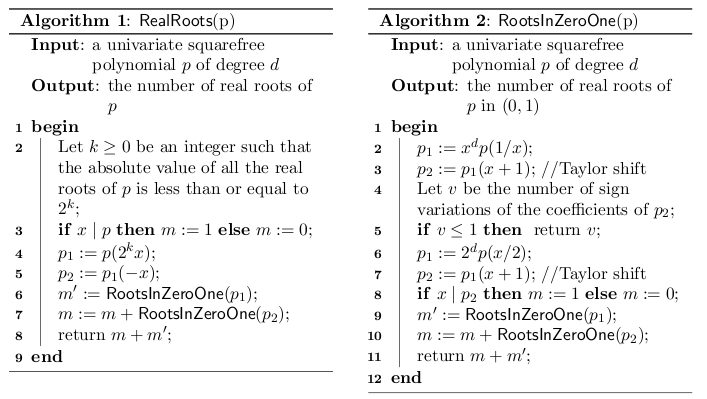
\includegraphics[scale = 0.2]{VCAalgo.png}
\end{center}

\begin{block}{}
The algorithm 2 is called several times and inside it, \textit{Taylor shift by $1$} also\\
\textcolor{blue}{\underline{$\Longrightarrow :$} \textit{Taylor shift by $1$} needs to be optimized at the lowest cost possible.}
\end{block}

\end{frame}
%%%%%%%%%%%%%%%%%%%%%%%%%%%%%%%%%%%%%%%%%%%%%%%%%%%%%%%%%%%%%%%%%

%%%%%%%%%%%%%%%%%%%%%%%%%%%%%%%%%%%%%%%%%%%%%%%%%%%%%%%%%%%%%%%%%
\begin{frame}[fragile]
\frametitle{\textbf{\textcolor{orange}{Modular arithmetic}}}

\begin{block}{}
\textcolor{darkgreen}{\textbf{A current problem :}} expressions in the coefficients swell when computing with polynomial or matrices over a field ($\mathbb{Z}$ e.g.) $\Rightarrow$ performance bottleneck for computer algebra.\\
\end{block}
\vline

\begin{block}{}
\textcolor{blue}{\textbf{Two solutions :}}
\begin{itemize}
\item use highly optimized multiprecision libraries (e.g. {\sc Gmp}), and
\item compute by \textcolor{red}{homomorphic images}.
\end{itemize}
\end{block}

\begin{block}{}
\textcolor{violet}{\textbf{Ways to compute by homomorphic images :}}
\begin{itemize}
\item use the \textcolor{red}{\textit{Chinese Remainder Theorem}}, or
\item use the \textit{Hensel's Lemma}.
\end{itemize}
\end{block}

\end{frame}
%%%%%%%%%%%%%%%%%%%%%%%%%%%%%%%%%%%%%%%%%%%%%%%%%%%%%%%%%%%%%%%%%

%%%%%%%%%%%%%%%%%%%%%%%%%%%%%%%%%%%%%%%%%%%%%%%%%%%%%%%%%%%%%%%%%
\begin{frame}[fragile]
\frametitle{\textbf{\textcolor{orange}{Chinese Remainder Theorem (1)}}}

\begin{crt1}
Consider $m_1$, $m_2$, \ldots, $m_r$ a sequence of $r$ positive integers which are pairwise coprime. Consider also a sequence $(a_i)$ of integers and the following system $(S)$ of congruence equations :
\begin{center}
$(S) : \begin{cases}
x \equiv a_1 \mod m_1 \\
x \equiv a_2 \mod m_2 \\
\;\;\;\;\vdots \\
x \equiv a_r \mod m_r
\end{cases}$
\end{center}

Then $(S)$ has a unique solution modulo $M = m_1\times m_2\times \dots \times m_r$ :

$$\textcolor{red}{x = a_1 \times M_1 \times y_1 + a_2 \times M_2 \times y_2 + \dots + a_r \times M_r \times y_r}$$

with $\forall i \in \mbox{\textlbrackdbl} 1, r\mbox{\textrbrackdbl}$, $M_i = \cfrac{M}{m_i}$ and $y_i\times M_i \equiv 1 \mod m_i$.
\end{crt1}

\end{frame}
%%%%%%%%%%%%%%%%%%%%%%%%%%%%%%%%%%%%%%%%%%%%%%%%%%%%%%%%%%%%%%%%%

%%%%%%%%%%%%%%%%%%%%%%%%%%%%%%%%%%%%%%%%%%%%%%%%%%%%%%%%%%%%%%%%%
\begin{frame}[fragile]
\frametitle{\textbf{\textcolor{orange}{Chinese Remainder Theorem (2)}}}

\begin{Lemma}
Let $f \in \mathbb{Z}[x]$ be nonzero of degree $n\in\mathbb{N}$ and $a\in \mathbb{Z}$. If the coefficients of $f$ are absolutely bounded by $B\in\mathbb{N}$, then the coefficients of $g=f(x+a)\in\mathbb{Z}[x]$ are absolutely bounded by $B(|a|+1)^n$.
\end{Lemma}

Our future results will be given in $\mathbb{Z}[x]/M\mathbb{Z}$. Thanks to lemma, if $M$ is sufficiently big, we could consider our results in $\mathbb{Z}[x]$. The algebraic form of the \textit{Chinese Remainder Theorem} will be also used for \textit{homomorphic images} :

\begin{crt2}
Let us consider $m_1,\,m_2,\,...,\, m_r$ a sequence of $r$ positive integers which are pairwise coprimes and $M = m_1\times m_2\times \dots \times m_r$. Then :
 $$\textcolor{red}{\mathbb{Z}/M\mathbb{Z} \cong \mathbb{Z}/m_1\mathbb{Z} \times \mathbb{Z}/m_2\mathbb{Z} \times \dots \times \mathbb{Z}/m_r\mathbb{Z}}$$
\end{crt2}

\end{frame}
%%%%%%%%%%%%%%%%%%%%%%%%%%%%%%%%%%%%%%%%%%%%%%%%%%%%%%%%%%%%%%%%%
